\chapter{Transformaciones en el disco}
\label{cap:angular}

Este capítulo se centra en analizar las funciones holomorfas del disco en sí mismo como transformaciones. Con esta nomenclatura queremos remarcar cómo se transforman distintos subconjuntos (discos centrados en el origen, en un punto arbitrario o tangentes al borde) cuando se aplica una función holomorfa. Para abordar el problema en discos a distancia positiva del borde usamos resultados clásicos, introducimos una distancia apropiada y la correspondiente interpretación asociada. Para estudiar las transformaciones de los horodiscos (o discos tangentes en un punto del borde) precisaremos el uso de derivadas angulares. Con las nociones de límite y derivada angular comenzamos el capítulo. \\

\section{Derivada angular}

\begin{definition}
    Un sector de $\disk$ en un punto $w \in \partial \disk$ es la región entre dos líneas rectas en $\disk$ que parten de $w$ y son simétricas con respecto  al radio que une $w$ con $0$.
\end{definition}

Así, si $f$ es una función definida en $\disk$ y $w \in \partial \disk$, entonces
    \begin{equation}
        \angle \lim_{z \to w} f(z) = L
    \end{equation}
    significa que $f(z) \to L$ cuando $z \to w$ a través de cualquier sector de $w$. Cuando esto ocurre, decimos que $L$ es el límite angular de $f$ en $w$. \\

\begin{definition}
    Decimos que una función $f$ holomorfa del disco $\disk$ en sí mismo tiene derivada angular en $w \in \partial \disk$ si para algún $\eta \in \partial \disk$, el límite
    \begin{equation*}
        \angle \lim_{z \to w} \frac{\eta - f(z)}{w - z}
    \end{equation*}
    existe. Se dice que dicho límite es la derivada angular de $f$ en $w$ y lo denotamos por $\angle f'(w)$.
\end{definition}

Basándonos en estas nociones previas, la existencia de derivada angular de $f$ en $w$ implica que $f$ tiene límite radial $\eta$ en $w$. De hecho, también se da la posibilidad de que la derivada de $f$ tenga límite radial en $w$. \\

Enunciamos a continuación un resultado del libro \citet[capítulo 13]{conway2} que nos va a permitir hacer un refinamiento del Teorema de Fatou introducido en el Capítulo \ref{cap:fatou}. \\ % Corolario 5.5

\begin{corollary}
    Si $f \in \bholomorphic{\disk}$ tiene límite radial $\zeta$ en $w \in \partial \disk$, entonces $f$ tiene límite angular $\zeta$ en $w$.
\end{corollary}

Por el Teorema de Fatou sabemos que toda función $f \in \bholomorphic{\disk}$ tiene límite radial en casi todo punto del borde del disco, entonces también tendrá límite angular en casi todo punto del borde. \\

\section{Lema de Schwarz-Pick}

En esta sección vamos a estudiar un resultado que surge a partir del Lema de Schwarz cuando se le aplica un cambio conforme de variable. A continuación enunciamos el Lema de Schwarz, cuya demostración, bien conocida, omitimos. \\

\begin{theorem}[Lema de Schwarz]
    Sea $f: \disk \to \closedisk$ una función holomorfa en el disco $\disk$ tal que $f(0) = 0$. Entonces:
    \begin{enumerate}[(i)]
        \item $\abs{f(z)} \leq \abs{z}$ para todo $z \in \disk$.
        \item Además, si para algún $z \not = 0$ se verifica que $\abs{f(z)} = \abs{z}$ o $\abs{f'(0)} = 1$, entonces existe $\lambda \in \complex, \abs{\lambda} = 1$ tal que $f(z)=\lambda z$.
    \end{enumerate}
\end{theorem}

\begin{obs}
    El hecho de que $\abs{f(z)} \leq \abs{z}$ implica que si $r < 1$ y $z \in D(0,r)$, entonces $f(z) \in D(0,r)$. Es decir, $f(D(0,r)) \subset D(0,r)$. \\
\end{obs}

El resto de la sección está dedicada a mostrar el resultado análogo en el caso general, cuando el origen no es un punto fijo de $f$. Este resultado es conocido como Lema de Schwarz-Pick. \\ % aunque necesitaremos introducir una distancia apropiada en el disco para establecerlo.

La herramienta clave para deducir el Lema de Schwarz-Pick a partir del Lema de Schwarz es la familia de automorfismos $\{\alpha_p: p\in \disk\}$ dada por
\begin{equation*}
    \alpha_p (z) = \frac{p-z}{1 - \bar{p}z}
\end{equation*}
para todo $z \in \disk$. Todo automorfismo $\alpha_p$ intercambia el origen con $p$. Por tanto, si $p, q \in \disk$, la composición de $\alpha_p$ y $\alpha_q$ permite aplicar $p$ sobre $q$. En particular, esto asegura que el grupo de automorfismos del disco actúa transitivamente sobre $\disk$. \\

\begin{theorem}[Lema de Schwarz-Pick]
    Si $f$ es holomorfa del disco $\disk$ en sí mismo, entonces para cualquier par de puntos $p, q \in \disk$, se tiene que
    \begin{equation*}
        \abs{\frac{f(q) - f(p)}{1 - \xbar{f(p)}f(q)}} \leq \abs{\frac{q-p}{1 - \xbar{p}q}}.
    \end{equation*}

    Además, se verifica la igualdad para algún par de puntos si y solo si se da la igualdad para todos los pares. Esto ocurre si y solo si $f$ es un automorfismo del disco unidad.
\end{theorem}

\begin{proof}
    Observamos que si $f(p) = 0$, para $p = 0$ se obtiene el Lema de Schwarz. En otro caso, sea $b = f(p)$ y tomemos la aplicación $\alpha_b \circ f \circ \alpha_p$, que lleva el disco en sí mismo fijando el origen. Si aplicamos el Teorema de Schwarz a esta aplicación, evaluando en el punto $z = \alpha_p(q)$, y observando que el automorfismo $\alpha_p$ es su propia inversa, tenemos la siguiente inecuación
    \begin{equation*}
        \abs{\alpha_b \circ f(q)} \leq \abs{\alpha_p(q)},
    \end{equation*}
    que es precisamente lo que queremos. La afirmación sobre la igualdad se sigue de la parte correspondiente del Lema de Schwarz. \\
\end{proof}

Esta generalización del Lema de Schwarz afirma que cualquier función holomorfa del disco $\disk$ en sí mismo que no sea un automorfismo, decrece estrictamente la distancia pseudo-hiperbólica, que introducimos a continuación. \\

\begin{definition}
    La distancia pseudo-hiperbólica entre dos puntos $p, q \in \disk$ viene dada por la siguiente expresión:
    \begin{equation*}
        d(p,q) = \abs{\alpha_p(q)} = \abs{\frac{p-q}{1 - \xbar{p} q}}.
    \end{equation*}
\end{definition}

Esta distancia es en realidad una métrica en $\disk$ que induce la topología euclídea usual. En particular, la distancia del origen a cualquier otro punto del disco es la euclídea. \\

\begin{figure}[!htbp]
    \begin{minipage}[h]{0.5\textwidth}
        \centering
        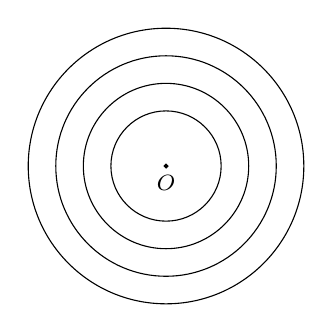
\begin{tikzpicture}[scale=0.35]
            \draw (0, 0) circle (2cm);
            \draw (0, 0) circle (3cm);
            \draw (0, 0) circle (4cm);
            \draw (0, 0) circle (5cm);
            \filldraw[black] (0, 0) circle (2pt) node[below, font=\footnotesize] {$O$};
        \end{tikzpicture}
        \label{fig:circulos1}
    \end{minipage} \hfill
     \begin{minipage}[h]{0.5\textwidth}
        \centering
        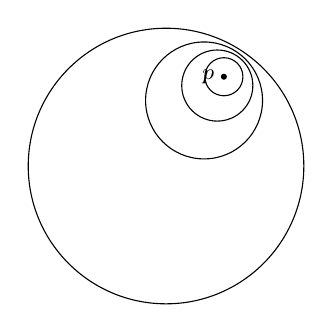
\begin{tikzpicture}[scale=0.35]
            \draw (0, 0) circle (5cm);
            \draw (2.1,3.24) circle (0.6905070600652824cm);
            \draw (1.86,2.92) circle (1.289961239727768cm);
            \draw (1.38,2.38) circle (2.121508896988179cm);
            \filldraw[black] (2.1, 3.24) circle (2.5pt) node[left, font=\footnotesize] {$p$};
        \end{tikzpicture}
        \label{fig:circulos2}
    \end{minipage}
    \caption{Imagen de discos concéntricos por el automorfismo $\alpha_p$.}
    \label{fig:automorfismo}
\end{figure}

La figura \ref{fig:automorfismo} muestra la imagen de discos concéntricos $D(0,r)$ mediante la función $\alpha_p$. Podemos observar que se trata de discos en $\disk$ que no tienen a $p$ como centro, salvo cuando aplicamos el único automorfismo que, salvo giros, conserva el centro, es decir, $\alpha_0$. \\

Para poder realizar una interpretación geométrica vamos a tener que estudiar los discos asociados con la distancia pseudo-hiperbólica. Si $p \in \disk$ y $0 < r < 1$, denotamos por $\Delta(p,r)$ al disco no euclídeo de (pseudo-) centro $p$ y (pseudo-) radio $r$ dado por $\Delta(p,r) = \alpha_p(D(0,r))$. Al ser $\alpha_p$ autoinversa se tiene que
\begin{equation*}
    \Delta(p,r) = \left\{z \in \disk: \abs{\frac{p-z}{1 - \xbar{p}z}} < r\right\} = \left\{z \in \disk: \abs{\alpha_p(z)} < r \right\}.
\end{equation*}

Con esta noción, el Lema de Schwarz-Pick se puede formular en los mismos términos geométricos en que interpretamos el Lema de Schwarz, referido a los discos no euclídeos $\Delta(p,r)$. \\

\begin{theorem}[Lema de Schwarz-Pick]
    Toda función holomorfa $f$ del disco $\disk$ en sí mismo lleva $\Delta(p,r)$ en $\Delta(f(p),r)$.
\end{theorem}

Observamos que si $p = 0$, tenemos que $f(D(0,r)) \subset D(0,r)$, que coincide con la interpretación geométrica del Lema de Schwarz. \\

\section{Teorema de Julia}

Con el Teorema de Julia se resuelve el equivalente al Lema de Schwarz-Pick para discos que no son interiores al disco unidad, sino tangentes en su borde. El punto de vista geométrico que deseamos destacar del Teorema de Julia nos conduce a describir estos discos tangentes en un punto $w$ del borde de $\disk$ a través de discos no euclídeos cuyos centros van aproximándose a ese punto $w$ en la frontera del disco unidad. \\

La pregunta natural en este ámbito se centra en la relación que deben guardar los centros $p_n$ y los radios $r_n$ para que la sucesión de discos $\{\Delta(p_n, r_n)\}$ converja (en el sentido adecuado) a un disco tangente. Observamos que cuanto más próximo esté $r_n$ al valor $1$, el disco $\Delta(p_n, r_n)$ es mayor, y el cociente entre las sucesiones $1 - \abs{p_n}$ y $1 - r_n$ determinará el tamaño del disco límite. Observando que
\begin{equation*}
    \abs{\frac{z-p}{1 - \xbar{p}z}} < r \Leftrightarrow 1 - r^2 < 1 -  \abs{\frac{z-p}{1 - \xbar{p}z}}^2 = \frac{(1-\abs{p}^2)(1-\abs{z}^2)}{\abs{1-\xbar{p}z}^2},
\end{equation*}
podemos describir los discos no euclídeos como
\begin{equation*}
\Delta(p,r) = \left\{z \in \disk : \abs{1-\xbar{p}z}^2 < \frac{1-\abs{p}^2}{1-r^2} (1-\abs{z}^2)\right\}.
\end{equation*}

Cuando $\lim_{n \to \infty} p_n = w$ y $\lim_{n \to \infty} \frac{1-\abs{p_n}^2}{1-r_n^2} = \lambda$, la expresión de la derecha de la desigualdad que define $\Delta(p_n, r_n)$ tiende a $\lambda(1 - \abs{z}^2)$, mientras que la de la izquierda tiende a $\abs{1 - \xbar{w}z}^2$. Todo ello nos conduce a la siguiente definición. \\

\begin{definition}
    Llamaremos horodisco en el punto $w$ y radio $\lambda$ al conjunto
    \begin{equation*}
        H(w,\lambda) = \{z \in \disk : \abs{1 - \xbar{w} z}^2 < \lambda(1 - \abs{z}^2)\}.
    \end{equation*}
\end{definition}

Es fácil comprobar que este horodisco coincide con el disco euclídeo $D(\frac{w}{1+\lambda}, \frac{\lambda}{1+\lambda})$. En particular, $H(w, \lambda)$ es tangente a la frontera del disco en el punto $w$. Un disco así aumenta de tamaño con $\lambda$ y ocupa el disco unidad cuando $\lambda \to \infty$. La figura \ref{fig:noeuclideos} muestra la evolución de $\Delta(p,r)$ cuando $p$ tiende a un punto $w$ de la frontera del disco. \\

\begin{figure}[!htbp]
    \begin{minipage}[h]{0.35\textwidth}
        \centering
        \begin{tikzpicture}[scale=0.35]
            \draw (0, 0) circle (5cm);
            \draw[fill=lavander] (0, 0) circle (3.6cm);
            \filldraw[black] (0, 0) circle (2.0pt) node[below, font=\footnotesize] {$O$};
        \end{tikzpicture}
        \label{fig:noeuclideo1}
        %\caption{$\Delta(0, r)$}
    \end{minipage} \hfill
    \begin{minipage}[h]{0.3\textwidth}
        \begin{tikzpicture}[scale=0.35]
            \draw (0, 0) circle (5cm);
            \draw[fill=lavander] (0.84,3.24) circle (1.1407015385279355cm);
            \filldraw[black] (0.8, 3.74) circle (2.5pt);
            \draw[color=black] (0.94, 4.11);
        \end{tikzpicture}
        \label{fig:noeuclideo2}
        %\caption{$\Delta(p_n, r_n)$}
    \end{minipage} \hfill
    \begin{minipage}[h]{0.3\textwidth}
        \begin{tikzpicture}[scale=0.35]
            \draw (0, 0) circle (5cm);
            \draw[fill=lavander] (2.299024850013829,3.0883087788941905) circle (1.1500204535309522cm);
            \filldraw[black] (3, 4) circle (2.5pt);
        \end{tikzpicture}
        \label{fig:noeuclideo3}
        %\caption{$H(w, \lambda)$}
    \end{minipage}
    \caption{Discos no euclídeos: $\Delta(0, r)$, $\Delta(p_n, r_n)$ y $H(w, \lambda)$.}
    \label{fig:noeuclideos}
\end{figure}

El Lema que presentamos a continuación es la herramienta que se precisa para obtener el Teorema de Julia. \\

\begin{lemma}[de Convergencia de Discos]
    Sean $w \in \partial \disk$, $\{p_n\} \in \disk$ y  $\{r_n\} \in (0,1)$ tales que  $\lim_{n \to \infty} p_n = w$ y $\lim_{n \to \infty} \frac{1-\abs{p_n}^2}{1-{r_n}^2} = \lambda$. Entonces,
    \begin{equation*}
        H(w, \lambda) = \{z \in \disk : z \in \Delta(p_n, r_n) \text{ para infinitos } n \in \naturals \} \subset \xbar{H(w, \lambda)}.
    \end{equation*}
\end{lemma}

En este punto podemos hacer uso del Lema de Convergencia de Discos para obtener una versión del Lema de Schwarz-Pick cuando los centros de los discos no euclídeos tienden a un punto del borde del disco unidad. \\

\begin{theorem}[de Julia]
    \label{th:julia}
    Si $f$ es una función holomorfa del disco $\disk$ en sí mismo no constante, y existen $w, \mu \in \partial \disk$ y una sucesión $\{p_n\} \in \disk$ que verifican
    {
    \leqnomode
    \setlength{\jot}{10pt}
    \setlength{\mathindent}{25pt}
    \setcounter{align}{0}
    \renewcommand{\thealign}{\alph{align}}
    \begin{align}
        & \lim_{n \to \infty} p_n = w;
        \alignno \label{eq:condjulia1} \\
        & \lim_{n \to \infty} f(p_n) = \mu;
        \alignno \label{eq:condjulia2} \\
        & \lim_{n \to \infty} \frac{1-\abs{f(p_n)}}{1-\abs{p_n}} = \delta < \infty.
        \alignno \label{eq:condjulia3}
    \end{align}
    }
    Entonces se cumple que
    {
    \leqnomode
    \setlength{\jot}{10pt}
    \setlength{\mathindent}{25pt}
    \setcounter{align}{0}
    \begin{align}
        & \delta > 0;
        \alignno \label{eq:julia1} \\
        & f(H(w, \lambda)) \subseteq H(\mu, \lambda \delta), \text{ para todo } \lambda > 0;
        \alignno \label{eq:julia2} \\
        & \angle \lim_{z \to w} f(z) = \mu.
        \alignno \label{eq:julia3}
    \end{align}
    }

    Además, si se da la igualdad en \eqref{eq:julia2} para algún $\lambda > 0$, entonces $f$ es un automorfismo del disco.
\end{theorem}

\begin{proof}
    \eqref{eq:julia1} Cuando $f(0) = 0$, el Lema de Schwarz prueba que $\abs{f(z)} \leq \abs{z}$ y así $\frac{1-\abs{f(p_n)}}{1-\abs{p_n}} \geq 1$, de donde $\delta \geq 1$. En el caso general, puesto que
    \begin{equation*}
        d(f(p), f(0)) \leq d(p,0) = \abs{p},
    \end{equation*}
    para todo $p \in \disk$. Se deduce fácilmente que
    \begin{equation*}
        \frac{\abs{1-\xbar{f(p)} f(0)}^2}{1-\abs{f(0)}^2} \leq \frac{1 - \abs{f(p)}^2}{1 - \abs{p}^2}.
    \end{equation*}

    Por la desigualdad triangular, tenemos
    \begin{equation*}
        \frac{1 - \abs{f(0)}}{1 + \abs{f(0)}} \leq \frac{\abs{1-\xbar{f(p)} f(0)}^2}{1-\abs{f(0)}^2}
    \end{equation*}

    Combinando las dos desigualdades y particularizando en $p_n$ se tiene
    \begin{equation*}
        \frac{1 - \abs{f(0)}}{1 + \abs{f(0)}} \leq \frac{1 - \abs{f(p_n)}^2}{1 - \abs{p_n}^2} \to \delta,
    \end{equation*}
    de donde se deduce que $\delta \geq \frac{1 - \abs{f(0)}}{1 + \abs{f(0)}} > 0$. \\

    \eqref{eq:julia2} La demostración se basa en el Lema de convergencia de discos. Fijemos $0 < \lambda < \infty$. Podemos suponer que $1 - \abs{p_n} < \lambda$, para todo $n$ (si $\lambda \geq 1$ es evidente, mientras que si $\lambda < 1$ se tiene también puesto que $\abs{p_n} \to 1^-$, excluyendo una cantidad finita de términos de $\{p_n\}$). Por lo que si tomamos una sucesión cuyo término general es
    \begin{equation*}
        r_n = 1 - \frac{1 - \abs{p_n}}{\lambda},
    \end{equation*}
    estará dentro del intervalo abierto $(0,1)$, $r_n \to 1$, y la sucesión
    \begin{equation*}
        \left\{\frac{1 - \abs{p_n}}{1 - r_n}\right\}
    \end{equation*}
    será constante con límite $\lambda$, para todo $n$. Así que la sucesión de discos no euclídeos $\{\Delta(p_n, r_n)\}$ satisface las hipótesis del Lema de Convergencia de Discos. \\

    Por la hipótesis \eqref{eq:condjulia3}, tenemos que
    \begin{equation*}
        \lim_{n \to \infty} \frac{1-\abs{f(p_n)}}{1-r_n} = \lambda \lim_{n \to \infty} \frac{1-\abs{f(p_n)}}{1-\abs{p_n}} = \lambda \delta,
    \end{equation*}
    y los discos $\Delta(f(p_n), r_n)$ también están bajo las hipótesis del Lema de Convergencia de Discos, para todo $n$. \\

    El lema asegura que si $z \in f(H(w, \lambda))$, entonces $z \in f(\Delta(p_n, r_n))$ para infinitos $n \in \naturals$ y, por el Lema de Schwarz-Pick, $z \in \Delta(f(p_n), r_n)$ para infinitos $n \in \naturals$. De nuevo el Lema de Convergencia de Discos garantiza que $z \in \xbar{H(\mu, \lambda \delta)}$. Como $f$ no es constante, $f$ es abierta así que se tiene $f(H(w, \lambda)) \subset H(\mu, \lambda \delta)$. \\

    \eqref{eq:julia3} Finalmente, debemos probar que todo entorno usual de $\mu$ contiene la imagen por $f$ de un entorno angular de $w$. Supongamos que tenemos un sector $S$ con vértice en $w$. Dado $\varepsilon > 0$, tomamos $\lambda > 0$ tal que $H(\mu, \lambda \delta) \subset D(\mu, \varepsilon)$. Podemos elegir $\rho > 0$ tal que $S \cap D(w, \rho) \subset H(\mu, \lambda)$. Por la parte \eqref{eq:julia2}, se tiene que $f(H(w, \lambda)) \subset H(\mu, \lambda \delta)$, lo que completa la prueba. \\
\end{proof}

Veamos con un par de ejemplos qué tipo de condición impone \eqref{eq:condjulia3} sobre el modo en que la imagen de $f$ se acerca al borde del disco. Vamos a observar que en el ejemplo \ref{ex:jul1} los cocientes valen siempre lo mismo, mientras que en el ejemplo \ref{ex:jul2} la imagen se aparta del borde cerca del punto $1$. Esto es debido a que en el segundo caso se trata de funciones donde el cociente \eqref{eq:condjulia3} no está acotado. Esto lleva asociado que exista o no la derivada angular de la función en el límite angular de la función. \\

\begin{example}
    \label{ex:jul1}
    La función
    \begin{equation*}
        f(z) = \frac{1 + z}{2}
    \end{equation*}
    tiene cocientes tipo \eqref{eq:condjulia3} acotados para toda sucesión $\{p_n\}$ que converja a $1$. De hecho, si cada $p_n > 0$ los cocientes valen exactamente $\frac{1}{2}$, que es la derivada angular de $f$ en el punto $1$. \\
\end{example}

\begin{example}
    \label{ex:jul2}
    Tomemos la siguiente función
    \begin{equation*}
        g = \sigma^{-1} \circ \phi_a \circ \sigma,
    \end{equation*}
    donde $\sigma$ es la transformación de Möbius $\sigma(z) = \frac{1+z}{1-z}$ (que lleva $1$, $i$ y $-1$ en $\infty$, $i$ y $0$, respectivamente, y aplica el disco unidad en el semiplano $\{z \in \complex : \Re z > 0\}$) y $\phi_a(z) = z^a, a \in (0,1)$. \\

    La función $g$ tiene límite $1$ en el punto $1$ y es tal que su imagen se aparta del borde de $\disk$ cerca del punto $1$, es decir, los cocientes de \ref{eq:condjulia3} no están acotados. \\

    La figura \ref{fig:ejemplo} muestra cómo se transforma el disco mediante la aplicación $g$. Dado que tanto $\sigma$ como $\sigma^{-1}$ son transformaciones conformes y, como hemos estudiado anteriormente, transforman circunferencias y rectas en circunferencias y rectas, la imagen de $g$ debe ser la región limitada por los arcos de circunferencia $\gamma_1$ y $\gamma_2$, que forman con el eje real un ángulo de $\frac{a \pi}{2}$ y $\frac{-a \pi}{2}$, respectivamente. \\

    \begin{figure}[!htbp]
        \centering
        \begin{tikzpicture}[scale=1.2]
            \draw[fill=cccccc,fill opacity=0.35] (0,0) circle (1cm);
            \filldraw (-1, 0) circle (1pt);

            \draw[->] (1.5, 0) -- (2.5, 0) node[midway, above, font=\footnotesize]{$\sigma$};

            \draw (3, -1) -- (3, 1);
            \fill[color=cccccc,fill=cccccc,fill opacity=0.35] (4.25, 1) -- (3, 1) -- (3, -1) -- (4.25, -1) -- cycle;
            \filldraw (3, 0) circle (1pt); 1.25

            \draw[->] (3.625, -1.5) -- (3.625, -2.5) node[midway, right, font=\footnotesize]{$\phi_a$};

            \draw (3, -2.75) -- (3, -5.25);
            \draw (4.25, -2.75) -- (3, -4);
            \draw (3, -4) -- (4.25, -5.25);
            \fill[color=cccccc,fill=cccccc,fill opacity=0.35] (4.25, -2.75) -- (3, -4) -- (4.25, -5.25) -- cycle;
            \filldraw (3, -4) circle (1pt);

            \draw[->] (0, -1.5) -- (0, -2.5) node[midway, left, font=\footnotesize]{$\sigma^{-1}\circ \phi_a \circ \sigma$};

            \draw (0, -4) circle (1cm);
            \draw [shift={(0, -5.05)}, fill=cccccc, fill opacity=0.35]  plot[domain=0.8097835725701668:2.3318090810196264,variable=\t]({1.45*cos(\t r)},{1.45*sin(\t r)});
            \draw [shift={(0, -2.95)}, fill=cccccc, fill opacity=0.35]  plot[domain=3.95137622615996:5.4734017346094195,variable=\t]({1.45*cos(\t r)},{1.45*sin(\t r)});
            \node[font=\footnotesize] at (0, -3.4) {$\gamma_1$};
            \node[font=\footnotesize] at (0, -4.6) {$\gamma_2$};
            \filldraw (-1, -4) circle (1pt);

            \draw[<-] (1.5, -4) -- (2.5, -4) node[midway, above, font=\footnotesize]{$\sigma^{-1}$};
        \end{tikzpicture}
        \caption{Transformación del disco mediante la función $g$.}
        \label{fig:ejemplo}
    \end{figure}

    La figura \ref{fig:lente} muestra, a su vez, la representación de la función $g$ mediante la técnica del coloreado. Estas funciones se suelen llamar \textit{lenticulares} ya que la imagen del disco es como una lente. Podemos observar todos los colores, pero bastante oscuros, salvo en los puntos $1$ y $-1$ que tienen la intensidad usual. \\

    \begin{figure}[!htbp]
        \centering
        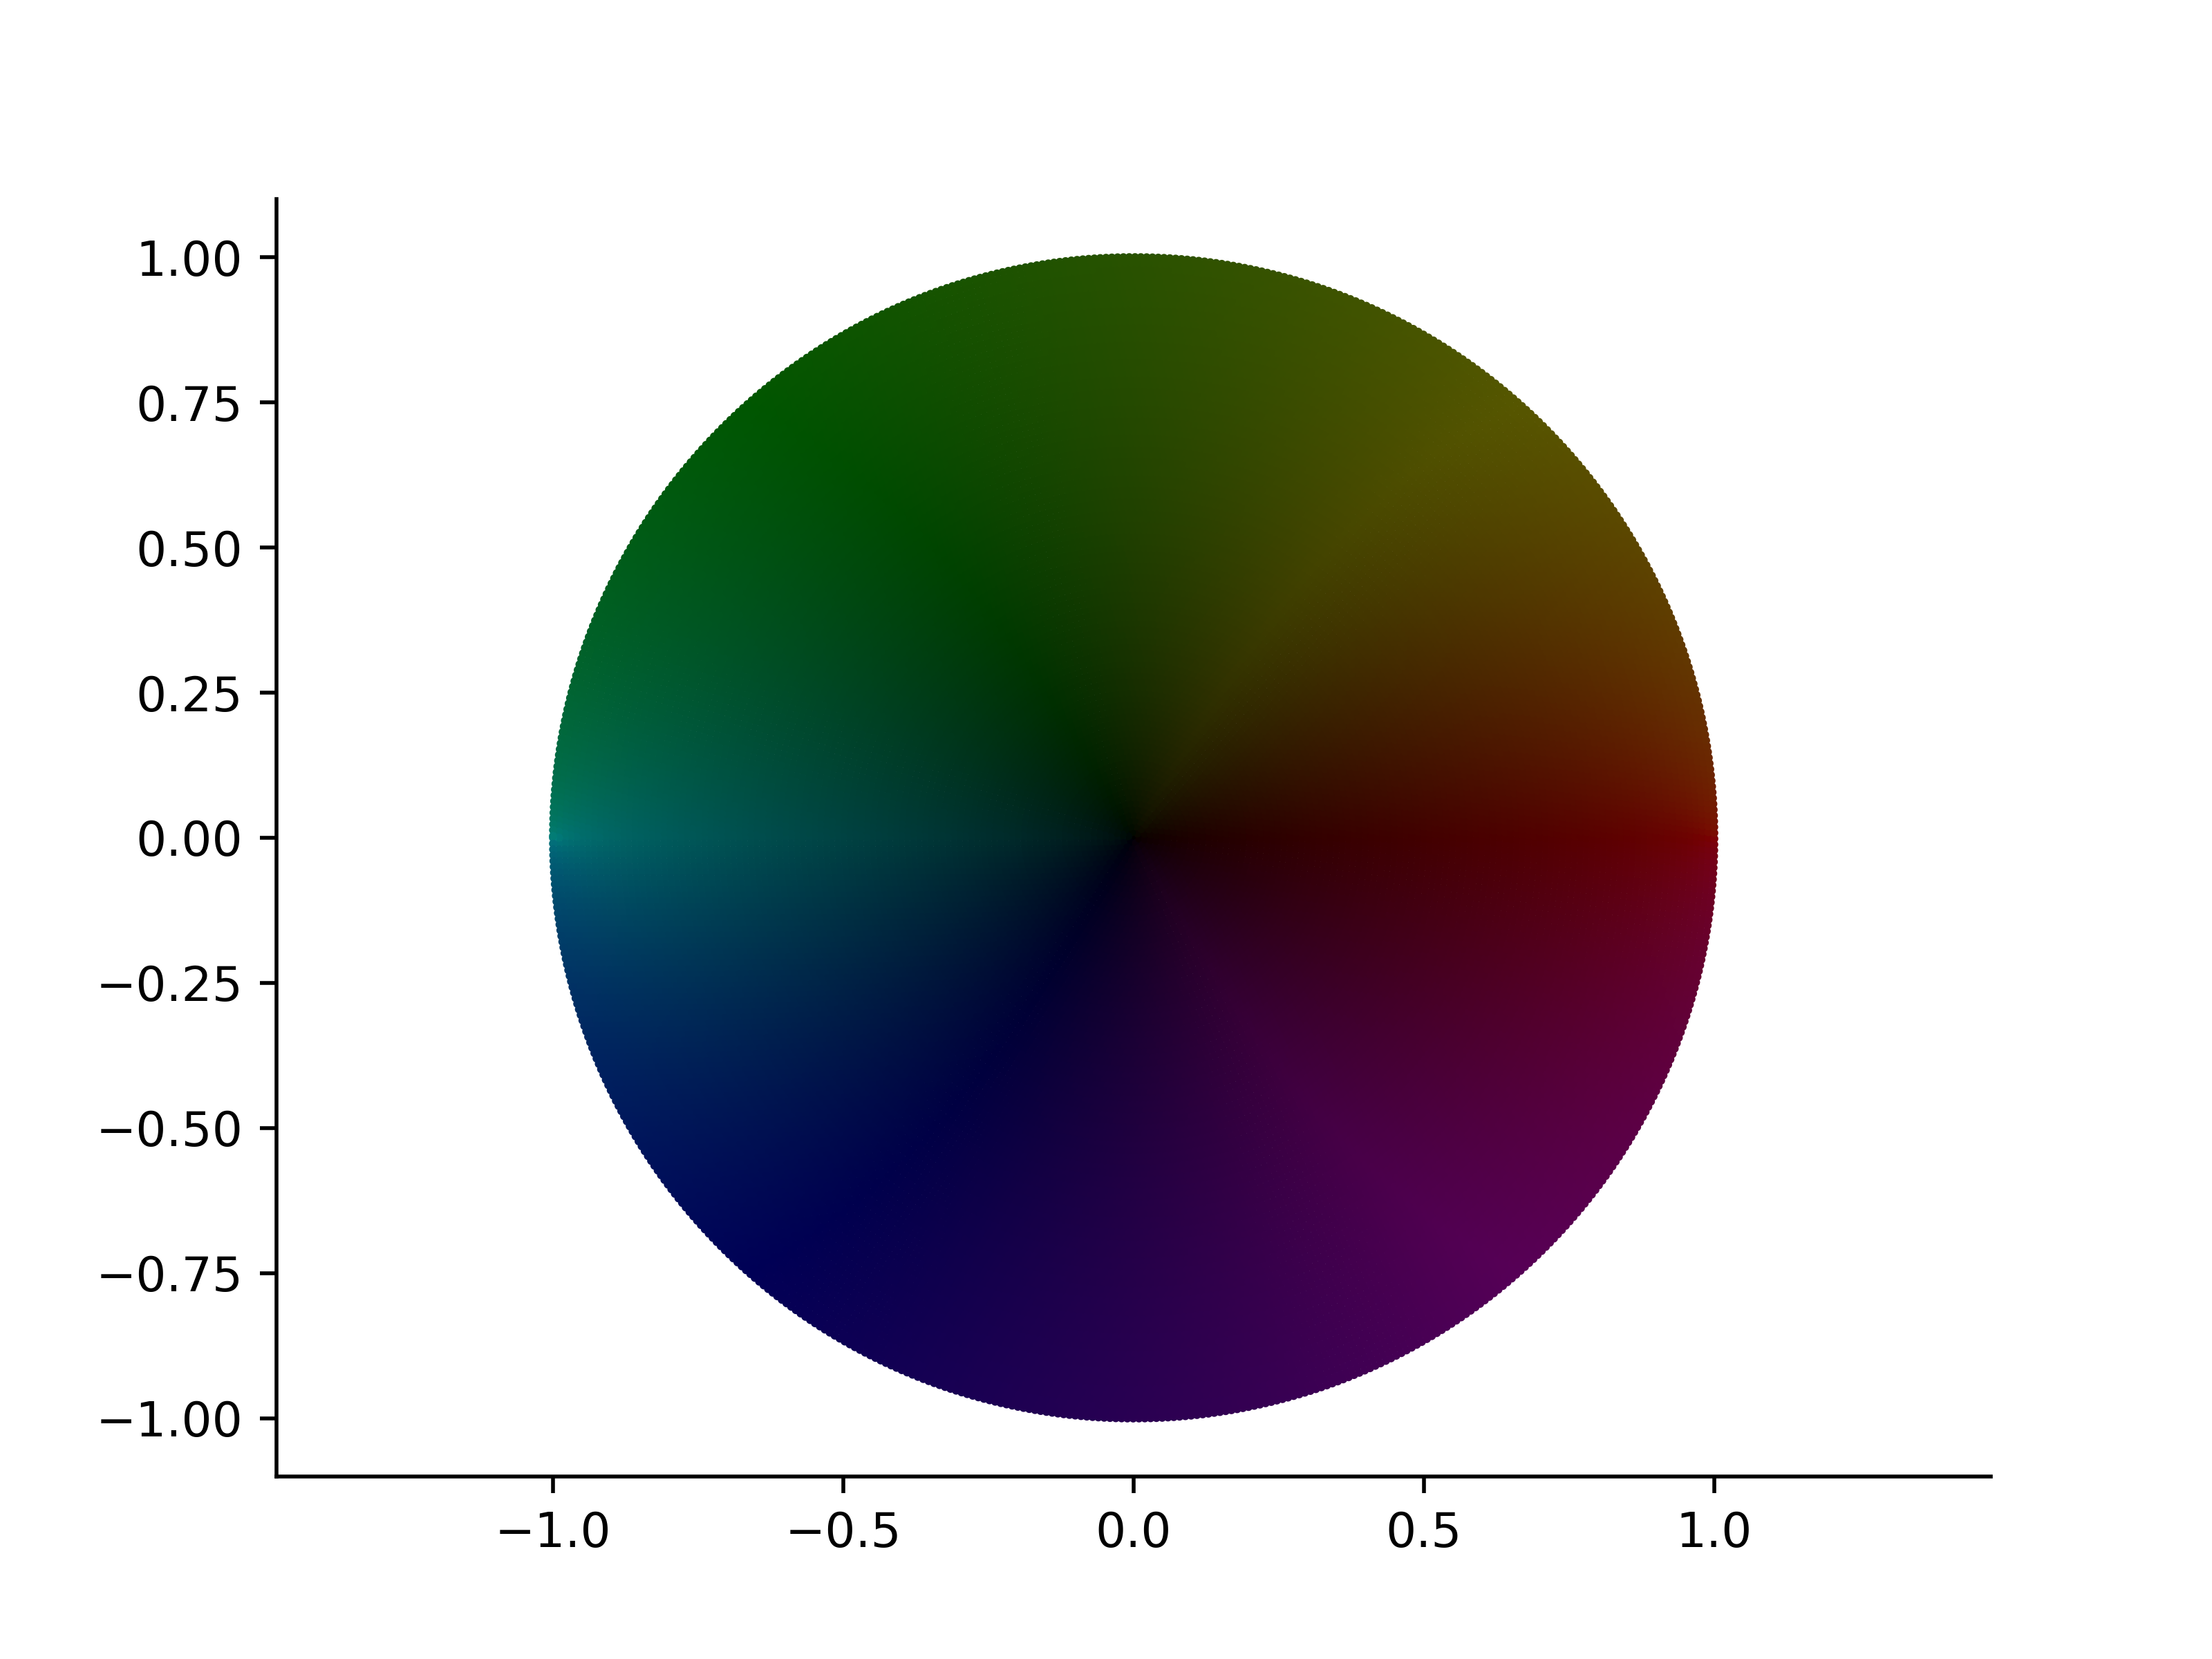
\includegraphics[width=0.7\textwidth]{../Aplicacion/lente.png}
        \caption{Representación de la función $g = \sigma^{-1} \circ \phi_a \circ \sigma$, con $a = \frac{1}{2}$.}
        \label{fig:lente}
    \end{figure}

    \begin{comment}
    La tabla \ref{tab:ejemplo} muestra, a su vez, los valores de los cocientes de tipo \eqref{eq:condjulia3} para la sucesión $p_n = 1 - \frac{1}{n}$ con $n = 10^2, 10^3, 10^6, 10^9$ y $10^{12}$ y distintos valores de $a$. En todos los casos, la sucesión $\{p_n\}$ verifica que $\lim_{n \to \infty} \frac{1-\abs{f(p_n)}}{1-\abs{p_n}} = \infty$ pero alcanza valores mayores más rápidamente a medida que $a$ sea menor y, por lo tanto, la imagen se aparta más del borde de $\disk$. \\

    \newcolumntype{g}{>{\columncolor{Gray}}c}
    \begin{table}[htpb]
        %\renewcommand*{\arraystretch}{1.5}
        \centering
        \begin{tabular}{|g|c|c|c|c|c|}
            \hline
            \rowcolor{Gray}
            $a$    & $n=100$   & $n=1000$  & $n=10^6$  & $n=10^9$       & $n=10^{12}$       \\ \hline
            $0,1$  & $7,40879$ & $637,231$ & $37973,6$ & $2,1\cdot10^8$ & $1,1\cdot10^{11}$ \\ \hline
            $0,5$  & $13,1774$ & $43,7325$ & $1413,21$ & $44720,3$      & $1414212$         \\ \hline
            $0,9$  & $1,67686$ & $2,13522$ & $4,26679$ & $8,51339$      & $16,9864$         \\ \hline
            $0,99$ & $1,04375$ & $1,07785$ & $1,15613$ & $1,23882$      & $1,32738$         \\ \hline
        \end{tabular}
        \caption{Valores de los cocientes de tipo \eqref{eq:condjulia3} para la sucesión $p_n = 1 - \frac{1}{n}$.}
        \label{tab:ejemplo}
    \end{table}
    \end{comment}

\end{example}

En $1929$, Carathéodory, probó que bajo las hipótesis del Teorema de Julia, la derivada también admite límite radial en dicho punto del borde. A continuación enunciamos sin demostración el teorema de Julia-Carathéodory. \\

\begin{theorem}[de Julia-Carathéodory]
    Sea $f$ es una función holomorfa del disco $\disk$ en sí mismo y sea $w \in \partial \disk$. Entonces las siguientes afirmaciones son equivalentes:
     {
    \leqnomode
    \setlength{\jot}{10pt}
    \setlength{\mathindent}{20pt}
    \setcounter{align}{0}
    \begin{align}
        & \liminf_{z \to w} \frac{1 - \abs{f(z)}}{1 - \abs{z}} = \delta < \infty;
        \alignno \label{eq:juliacar1} \\
        & \lim_{z \to w} \frac{\eta - f(z)}{w - z} \text{ existe para algún } \eta \in \partial \disk;
        \alignno \label{eq:juliacar2} \\
        & \angle \lim_{z \to w} f'(z) \text{ existe y } \angle \lim_{z \to w} f(z) = \eta \in \partial \disk.
        \alignno \label{eq:juliacar3}
    \end{align}
    }
\end{theorem}

Además, $\delta > 0$ en \eqref{eq:juliacar1}; los puntos del borde $w$ y $\eta$ de \eqref{eq:juliacar2} y \eqref{eq:juliacar3} son los mismos; y $\angle \lim_{z \to w} f'(z) = \angle f'(w) = w \xbar{\eta} \delta.$ \\

Después de las rotaciones preliminares apropiadas, se puede suponer que $w = \eta$. Por lo tanto, estos resultados muestran que si $f$ tiene una derivada angular en algún punto del borde $w$ tal que $\angle \lim_{z \to w} f(z) = w$, y $\angle f'(w) < 1$, entonces $ f $ no puede tener un punto fijo en $\disk$. \\

Ahora supongamos únicamente que $f$ no tiene ningún punto fijo en $\disk$. La pregunta que nos hacemos es: ¿existe la derivada angular en un cierto punto del borde? La respuesta afirmativa fue dada por J. Wolff en $1926$. \\

A continuación presentamos el Teorema de Wolff que garantiza que toda función $f$ del disco en sí mismo sin puntos fijos lleva asociado un punto $w$ con $\abs{w} = 1$ tal que todo disco tangente en $w$ al borde del disco se aplica sobre sí mismo por $f$. \\

\begin{theorem}[de Wolff]
    Si $f$ es una función holomorfa del disco $\disk$ en sí mismo que no tiene puntos fijos, existe un único $w \in \partial \disk$ tal que
    \begin{enumerate}[a)]
        \item $\lim_{r \to 1} f(rw) = w$ ($w$ es un punto fijo en el borde).
        \item Para todo horodisco $H(w, \lambda)$ se tiene $f(H(w, \lambda)) \subset  H(w, \lambda)$.
    \end{enumerate}
\end{theorem}
